
In this section we talk about the context underlighing our contribution and present the motivations that lead to our approach.

\subsection{Context: Mobile Crowd-Sensing Platforms}

Preserving privacy in the mobile crowd-sensing platforms context is a key challenge to address.
The platforms must deal with users' privacy preserving and quality of data.
There is a balance to find between a the level of the users' privacy preserving and the quality of the data that are collected.
Indeed, if a crowd-sensing platform put a lot of consideration in the privacy preserving, the collected data could be degraded depending to the data type.



Users may not want to contribute in a sensing system if their privacy is engage.

Crowd-sensing platforms are systems that collect and aggregate knowledge from a large amount of devices.
APISENSE is one of these platform that provide to scientists an easy way to deploy their sensing experiments in the wild. By using these platforms they can test their theories on real data instead of simulated one.



These data come from users that subscribe to data collect campaign and contribute with their mobile devices.



%
Preserving privacy in the context of crowd-sensing platforms is a key challenge to address.
In particular, the anonymization of crowdsourced datasets is a priority when it comes to increase the privacy of end-users [4]. To the best of our knowledge, data anonymization techniques are often deployed on the server side [9], [6]. 
This observation can be correlated with the difficulty of developing mobile apps enabling peer-to-peer mobile communications. 
For example, none of Android or iOS emulators support proximity wireless interactions and the only
way is to test them is to use real devices. 
However, this method does not scale and cannot reproduce realistic events that can be encountered in real deployments. 
Another limitation in the geo-privacy field is the incapacity to reproduce and compare experiments. Geo-privacy focuses its interest on the critical impact of location data on users privacy. 
In this domains, the evaluation builds on shared datasets, which are used by the community to test
and assess their algorithms. However, these datasets are often altered for the purpose of evaluation and this modification of the input data prevents from further comparisons.
Finally, in the mobile computing community, some simulation tools give the opportunity to simulate many devices, network and others. However, these tools are not focused on crowd-sensing concerns like wireless proximity issues or the validation on a very large number of emulators running
and moving at the same time.
In this paper, we address these drawbacks by providing a data dissemination approach that leverages peer-to-peer communications on mobile device to anonymize data. 
Our approach take advantages of the privacy-by-design principles presented by Langheinrich [16].
We also describe the design of an emulation platform, which can be used to reproduce human movement with real location data and test crowd-sensing applications in more realistic settings.
%




The data anonymization is mad on the server side.

With this approach we must trust the centralized server.


Crowd-sensing platforms have a large application domain.
Applications encompass application performance monitoring (\emph{e.g.}, OpenSignal\footnote{\url{http://opensignal.com}}), environment monitoring (air quality\footnote{\url{http://citizensensor.cc}}), etc.


Currently, the system uses a centralized approach where each smartphone individually report data to a central server.

Datasets are anonymized \emph{a posteriori}~\cite{DBLP:conf/icdcs/PrimaultMB15}, which does not protect from malicious behaviors during the upload phase.

\subsection{Motivations: Data Dissemination Threats}

As exposed above, in APISENSE, a collect server can be managed by an external organization.
The way of having a single trusted server that handle all users data sending is not practicable.
Having multiple server is a requirement in this kind of platform and we can say that no server can be trusted.

A key challenge in the crowd-sensing platforms is to avoid central trusted server that present a single point of failure that need to be address.

Let imagine a user named Alice that participate to a data collect campaign.
Alice produces data and sends it directly to the central server.
In this scenario the server knows that Alice is the producer of the data that she sends.

Even if we have a strong trust in the central server about keeping users' data safe, this server is a target of choice for an attacker.
The security of the server can be compromized and users data can be stollen in a single attack on the server.
This kind of architecture is not safe because of its single rupture point.

Moreover, in the case of APISENSE architecture, collect servers can be maintain by other organizations that could keep informations about users before sending their data to the trusted central server.
This kind of treats is not acceptable in a privacy way.

To address this scenario, we think-off a method where user 

\begin{figure*}[t]
	\centering
	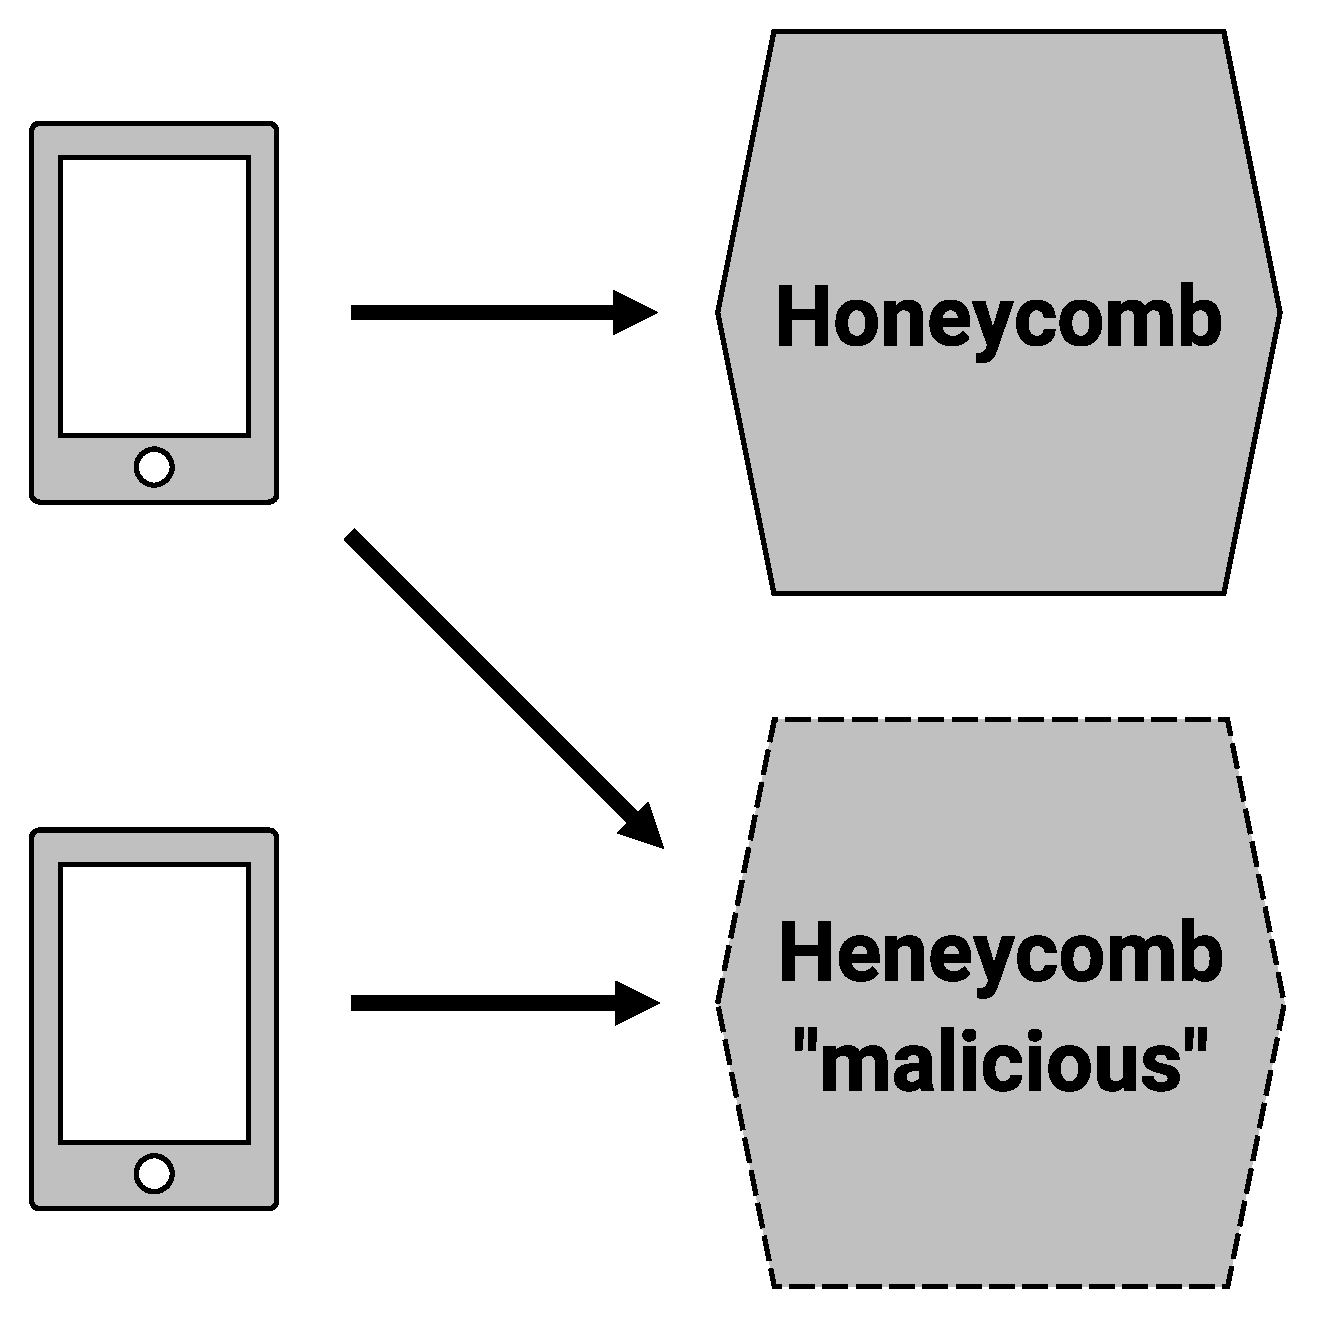
\includegraphics[width=0.4\textwidth]{figures/honeycomb}
	\caption{\label{Honeycomb} APISENSE data collection treat}
\end{figure*}

%%%% OK

\subsection{Goals: Enabling Decentralized Dissemination}

The main goal is to provide a decentralized data dissemination approach that could protect the users' privacy in an untrusted environment.
We want to trend to a solution that could take the advantages of a Privacy by design approach which leads to a minimal intrinsically privacy-preserving system.
Ultimately, our objective is to break the ability of an end-server to link a data to his producer without compromising the quality and the utility of the whole dataset.

%%%% END OK